\chapter{单相渗流LB模拟在GPU上的实现及优化}
上一章中计算所使用的算例流场边界都比较规则、简单,流场内部格点都是
流体格点,每个格点执行的操作都相同,线程中几乎没有逻辑判断分支语句。
这在GPU实现时意味着同一个Wrap中的各个线程执行路径完全相同,SP执行效率
最高,因此用LBM模拟这种简单流场流动时能充分发挥GPU的并行效率。但在模拟
实际问题时,流场结构通常并不规则,甚至非常复杂,如多孔介质。如何在GPU
上高效地实现这中复杂边界LBM模拟依然是当前的一个研究热点。
本章正是围绕这一问题探讨了从算法上考虑的各种优化途径,并以一个实际
多空介质流动(渗流)算例验证了优化效果。

\section{对于多孔介质的一般处理方法}
在多孔介质结构中,流体在相互连通的孔隙中流动,孔隙壁面是非规则的
固体表面。将多孔介质在空间上离散后,计算区域被划分为流体格点和固体格
点,如图\ref{fig:porous_2d}所示为二维多孔介质离散后的格点分布,图中黑色
格点表示固体,白色格子表示孔隙(流体)。在程序实现时用一个整型数组\verb+flag[NY][NX]+
来记录格点的类型,\verb+flag[y][x] = 0+表时格点\verb+(y,x)+为流体格点,等于
1则为固体格点,演化时通过这个数组判断格点类型,若为固体格点,则不作任何
处理。流固边界边界通常采用简单的标准反弹格式,处理时也需要判断周围格点类型。
\begin{figure}[htb]
  \centering
  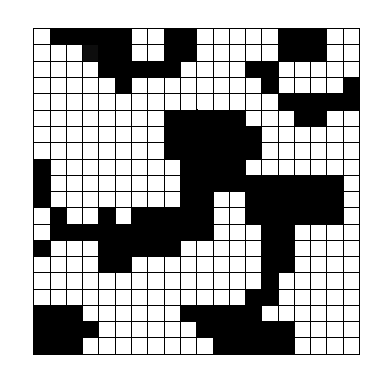
\includegraphics[width=0.6\textwidth]{img/porous_2d}
  \caption{二维多空介质示例}
  \label{fig:porous_2d}
\end{figure}

上述处理方式虽然实现起来简单,但在GPU上实现时效率不会很高。原因有二,
其一,处理每个格点时要周围格点类型,需要从全局内存加载周围格点
flag数据,占用了显存带宽,并且访存时存在第四章中所述显存地址
不对齐的情况;其二,确定周围格点类型时会引入判断分支
语句,如果一个wrap中的线程对应的格点既有流体格点,又有固体格点,
则会导致该wrap中的线程串行执行,执行效率将大为降低,在均匀的各向
同性介质中,这种情况将尤为明显,因为几乎每个wrap中都产生了分支。
上述方式除了在GPU上执行效率不高外,还存在另一个问题\--- 浪费存储
空间,因为在开辟PDF(速度分布函数)数组时,不参与计算的固体格点也占据了存储空间。
并且多孔介质的孔隙率越低,无效格点所占比例越高,存储空间浪费越严重。

%针对上述两个,我们分别采用两个方法解决
针对前一个问题,我们采用\textit{位存储模式}结合\textit{逻辑运算}方式解决,
针对第二个问题,我们采\textit{稀疏存储模式}解决。

另外,考虑到本文
最终目的是要做多组分模拟,我们在这里并没有采用第四章中所描述的使用共享内存
进行辅助迁移的方法,而是在碰撞之前从周围格点直接读取PDF。
之所以这样做,是因为在多组分模拟时,每个格点需要迁移的PDF几乎翻倍,
如果还是用共享内存辅助迁移,则SM的利用率会因共享内存数量限制而降低,进而
影响程序性能。Obrecht等人对这两种执行迁移步骤的方法做了详细对比,并指出
第二种方法在模拟复杂问题如非等温情况时,会比第一种方法效率更高\ucite{obrecht2011new}。

\section{优化技术一 ~ 位存储和逻辑运算} \label{sec:opt1}
因为每个格点只能是流体格点或固体格点,所以理论上在flag中只用一个bit就可以反映
格点类型。为了避免在演化过程中从加载周围格点的flag位,可以事先把这些
信息存储在当前格点的flag中。按这种方法,对于DnQq模型,每个格点的flag要存储$q$bit的信息,
其中$1$bit反映该格点本身类型,另外$(q-1)$bit反映周围格点类型。对于D3Q19模型,
可以用一个\texttt{int}类型($32$bit)来表示flag,如图\ref{fig:bitmap}所示,最低位
表示当前格点本身类型,第1到18位分别表示第1到18个方向上相邻格点的类型(0或1)。
\begin{figure}[htpb]
  \centering
  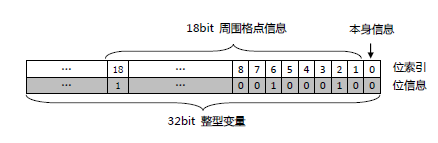
\includegraphics[]{img/bitmap}
  \caption{D3Q19模型falg的位存储模式示意}
  \label{fig:bitmap}
\end{figure}
利用这种位存储模式,解决了占用存储带宽的问题,接下来介绍利用逻辑运算来统一处理
内部流体格点和固体边界处流体格点的方法。

通常在处理流场内部格点和边界流体格点,程序会进入不同的分支语句。这里以修正反弹
格式为例,在这种反弹格式中,边界流体格点也需要执行碰撞,但它们与内部格点不同的是,
在从周围格点读取PDF时,如果该在该方向上临近格点是固体点,则从其本身的反方向读取PDF。
这里笔者提出一种能同一处理内部格点与边界格点的方法,这种方法可以保证同一个wrap中
各个线程执行的指令完全相同,指令吞吐量最高。代码\ref{code:opt2}示例了如何使用逻辑运算实现这种
方法。

\begin{Code}
\begin{lstlisting}
  ...
  //由于程序中使用了动态内存存储PDF
  //`所以用`GID`宏来做数组索引转换`
  //(z, y, x)格点(当前点)在一维数组中的位置
  k = GID(z,y,x); 
  flag_k = flag_h[k]; //当前点的flag
  //当前点为流体格点时才进行下面处理
  if(!(flag_k & 1)) 
  {
    ...
    for(i=1;i<Q;i++)  //读取各个方向上前一格点的PDF
    {
      //是否从本身读取PDF
      readShift = (flag_k & (1<<i)) == 0; 
      //`读取`PDF`的方向`
      i_reverse = i + (readShift^1)*((i&1)*2 - 1);
      xp = x - readShift*e[i_reverse][0];   
      yp = y - readShift*e[i_reverse][1];
      zp = z - readShift*e[i_reverse][2];
      kp = GID(zp, yp, xp);  
      //正式加载PDF
      F[i] = fIn[i_reverse*size + kp]; 
      ...
    }
  }
\end{lstlisting}  
\caption{优化技术一}
\label{code:opt2}
\end{Code}
如果周围格点时流体点则\texttt{readShift=1},表示读取位置有偏移,否则从自己读,
\texttt{readShift=0},没有偏移。如果读取位置有偏移,则从\texttt{i}方向的反
方向(\texttt{i\_reverse}读(此时\texttt{i\_reverse != i})。
因为我们在定义离散速度方向时,保持了第\texttt{i}个与第\texttt{i+1}个方向正好
相反(\texttt{i}为偶数),所以可以通过\texttt{i}的奇偶性判断其反方向。

值得注意的是上述优话指令流的方法也可以运用于其他需要避免\texttt{if}语句的地方,具有一定的
通用性。

\section{优化技术二 ~ 稀疏存储模式}\label{sec:opt2}
稀疏存储模式是指只存储流体格点PDF,目的是为了节省内存或显存(GPU程序),通常
GPU显存并不大(几GByte),因此在GPU程序中,这一方法更为重要。稀疏存储模式中,
首先遍历\texttt{flag}数组,统计出流体格点个数,然后动态分配一维线性内存/显存
存储流体格点PDF,流体格点的PDF按格点在遍历过程中出现的顺序插入该线性内存,如图\ref{fig:node_map}。
由于流体格点分布不规则,所以流体格点之间的相对位置关系丢失了,在迁移时不能确定
周围格点PDF的内存/显存地址。解决这个问题的办法是引入一个辅助数组来保存每个
格点各个方向上相邻格点在的位置,我们称这个数组为\texttt{node\_map}。在GPU上
实现时,\texttt{node\_map}按\texttt{node\_map[Q-1][num\_F]}形式存储数据,即依然
保证访问地址连续。
%流体格点之间的相对位置关系,
\begin{figure}[htpb]
  \centering
  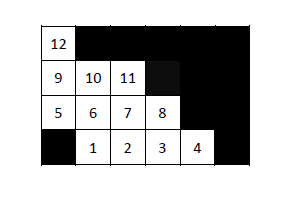
\includegraphics[]{img/node_map}
  \caption{稀疏存储模式}
  \label{fig:node_map}
\end{figure}
稀疏模式还有一个附加优点,因为在\texttt{node\_map}中直接存储了
\emph{每个周围格点的PDF}在PDF数组中的索引,这样可以在构造\texttt{node\_map}时
将反弹格点与周期边界格点的迁移源地址或目的地址地直接存在里面,
而在演化过程中不需要显示处理这些特殊格点,因而
Kernel函数大为简化。

引入辅助数组之后,虽然每个格点要存储的信息增多了,但在孔隙率低于某个阈值(
当PDF采用双精度时,该阈值约为为0.7)时
总的内存/显存用量仍低于全存储模式\ucite{pan2004high}。

值得指出的是,稀疏存储模式在CPU上和GPU上运用都可以节省存储空间,但在CPU
上相对于全存储模式并不会提高计算速度,而在GPU上却可以显著提高。这是
GPU和CPU构架差异造成的,当在GPU上运用全存储模式时,不参与计算的无效格点
占据了SP执行时间,而采用稀疏存储模式时,则不存在这一问题。本章后面
分析GPU程序性能将会验证这个现象。
%ADD 确定内存用量

\section{算例一 ~ BCC结构渗透率的测定}
\subsection{问题描述}
单相流体在外力或压差驱动下流过多孔介质时,其平均流速(达西速度)可由
达西定律给出
\begin{equation}
  u_d = -\frac{k}{\rho \nu}(\nabla p_z + \rho g)
  \label{darcy}
\end{equation}
其中$k$为多孔介质的渗透率,其具体值只有多孔介质结构本身确定,与其中
所通过的流体性质无关。本算例中使用的多孔介质模型BCC结构的渗透率具有
近似解析解,我们将其与数值模拟得出的渗透率对比来验证程序正确性。

BCC结构是指体心立方结构(Body Centered Cubic),它是一种理想多空介质
模型,其结构如图\ref{fig:bcc_array}所示,其中球体表示固体区域。因为球体
排布具有空间周期性,所以计算区域只取其一个基本单元,如图\ref{fig:bcc}所示,
其二维投影如图\ref{fig:bcc_2d}。
\begin{figure}[htpb]
  \centering
  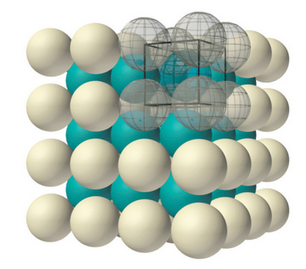
\includegraphics[]{img/bcc_array}
  \caption{BCC结构示意图}
  \label{fig:bcc_array}
\end{figure}

\begin{figure}[htb]
  \centering
  \subfigure[BCC结构基本单元]{
    \begin{minipage}[b]{0.4\textwidth}
      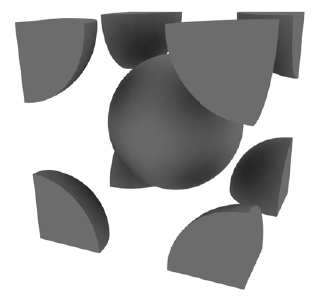
\includegraphics[width=1\textwidth]{img/bcc}
      \label{fig:bcc}
    \end{minipage}
  }
  \subfigure[BCC结构二维投影]{
    \begin{minipage}[b]{0.4\textwidth}
      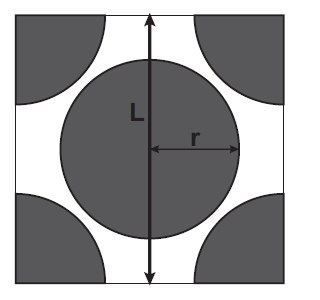
\includegraphics[width=1\textwidth]{img/bcc_2d}
      \label{fig:bcc_2d}
    \end{minipage}
  }
  \caption{BCC结构及参数}
\end{figure}
BCC结构参数为球体半径$r$和立方体单元边长$L$。固体区域所占体积比例与孔隙率分别是
\begin{equation}
  c=\frac{8\pi r^3}{L^3}, \quad \epsilon = 1-c
  \label{bcc_c}
\end{equation}
其中$c$的最大值为$c_{max} = \frac{\sqrt{3}\pi}{8}$,通常用一个取值范围为0到1的
无量纲形状因子$\chi = \left(\frac{c}{c_{max}}\right)^{1/3}$来表示球体填充的致密程度,$\chi=1$时填充
最为致密的情况,图\ref{fig:bcc}就是这种情况。
BCC结构的绝对渗透率近似解析解形式为
\begin{equation}
  k = \frac{2\epsilon r^2}{9d^*(1-\epsilon)}
  \label{k_ana}
\end{equation}
其中$d^*$是单个球体所受流体拖拽力的无量纲阻力,在$Re<1$的情况下其级数近似
解析解\ucite{sangani1982slow}为
\begin{equation}
  d^* = \sum\limits_{n=0}^{30}\alpha_n\chi^n
  \label{d_star}
\end{equation}
其中多项式系数$\alpha_n$为常数,具体值见参考文献\cite{sangani1982slow}。

\subsection{数值方法}
我们通过给定外力$g$,在流场稳定后测出达西速度$u_d$,然后根据式\eqref{darcy}得出
渗透率数值解。流场的所有外边界均为周期性边界,流固边界采用修正反弹格式,外力离散格式
采用Luo的二阶矩模型\ucite{luo1998unified}。模拟过程中保证$Re < 1$,网格规模均为$128^3$,
立方体尺寸为128m。计算收敛标准为计算所得渗透率相邻1000步的相对变化小于$10^{-5}$。如
无特别指明,所有工况在GPU上均用单精度计算。

Pan等人指出用LBGK模型计算多空介质介质流动时,
存在计算所得渗透率时与粘性相关的非物理现象,
而MRT模型可以显著改善这一问题\ucite{pan2006evaluation}。
这里我们也采用D3Q19 LBGK 和D3Q19 MRT模型并验证了这一现象。在程序实现时我们分别采用
了前两节所介绍的优化技术。

\subsection{计算结果}
%由于采用不同算法只影响计算结果而不影响计算结果,所以这里
\subsubsection{MRT与LBGK}
我们分别用LBGK和MRT模型计算了不同孔隙率和不同流体粘性对应的绝对渗透率。图\ref{fig:bcc_streamline}
和图\ref{fig:bcc_U}所示为$\chi = 0.8,\tau=0.8$时用LBGK计算得到的
流线图和沿外力方向的速度分布图。
\begin{figure}[htb]
  \centering
  \subfigure[流线图]{
    \begin{minipage}[b]{0.4\textwidth}
      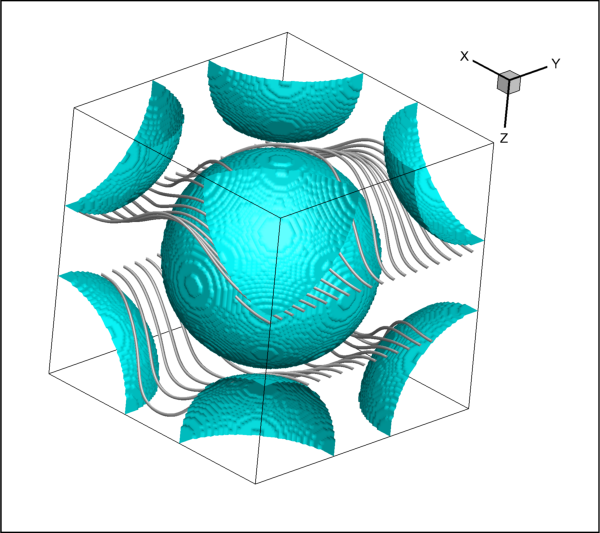
\includegraphics[width=1\textwidth]{img/bcc_streamline}
      \label{fig:bcc_streamline}
    \end{minipage}
  }
  \subfigure[沿外力方向的速度分量]{
    \begin{minipage}[b]{0.4\textwidth}
      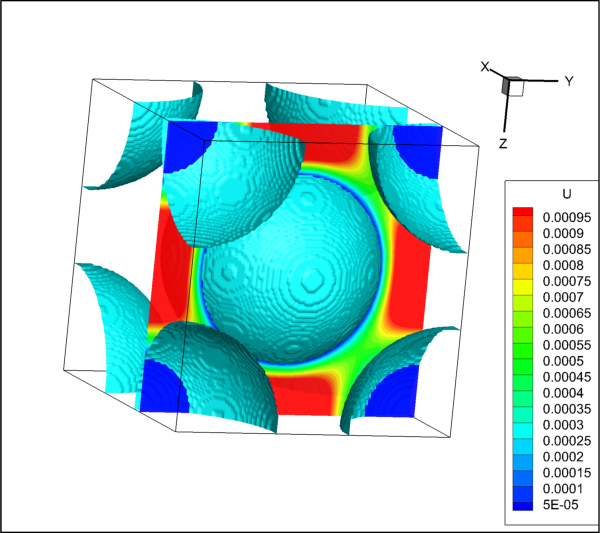
\includegraphics[width=1\textwidth]{img/bcc_U}
      \label{fig:bcc_U}
    \end{minipage}
  }
  \caption{LBGK模型$\chi=0.8, \tau=0.8$计算结果}
\end{figure}

\begin{figure}[htb]
  \centering
  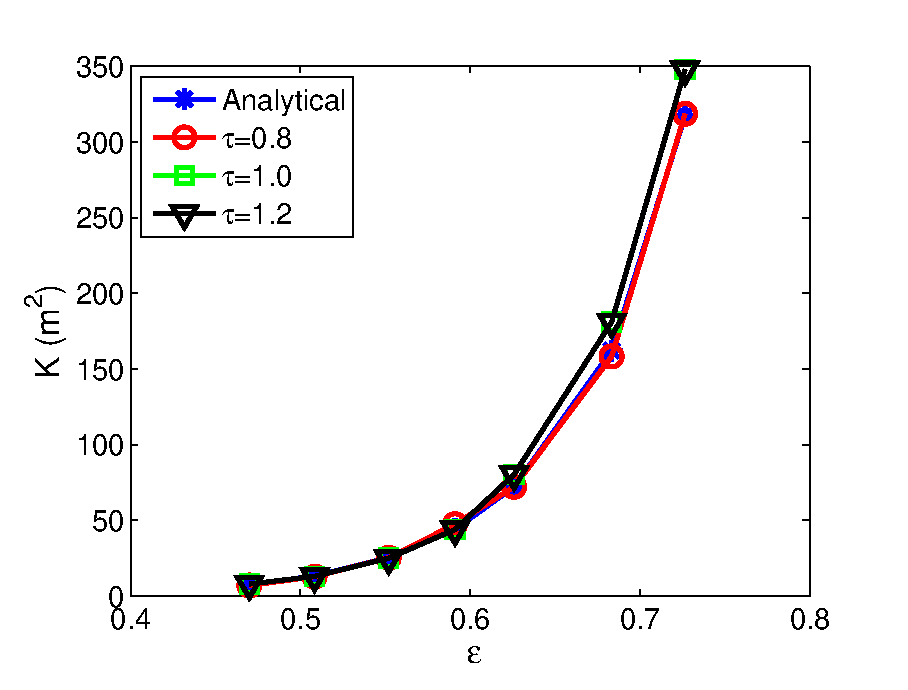
\includegraphics[width=0.6\textwidth]{img/k_bgk}
  \caption{使用LBGK模型时不同粘性和孔隙率下渗透率数值解}
  \label{fig:suckbgk}
\end{figure}

\begin{figure}[htb]
  \centering
  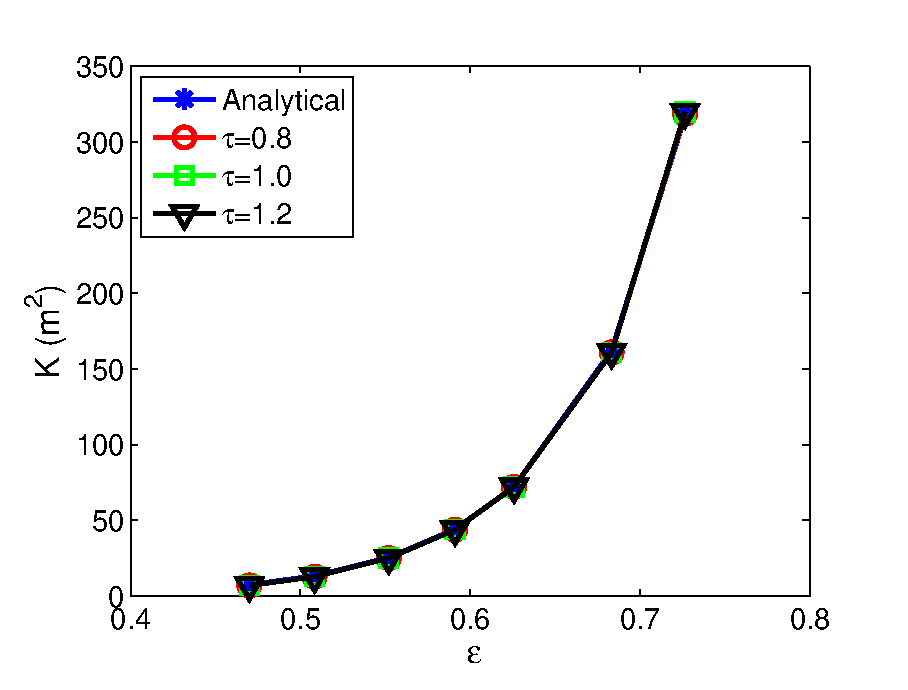
\includegraphics[width=0.6\textwidth]{img/k_mrt}
  \caption{使用MRT模型时不同粘性和孔隙率下渗透率数值解}
  \label{fig:suckmrt}
\end{figure}

图\ref{fig:suckbgk}和图\ref{fig:suckmrt}分别为不同孔隙率和不同流体粘性时计算得出的渗透率,
可以看出使用LBGK模型计算出来的渗透率会随粘性不同而变化明显,尤其是在孔隙率较高时,
而使用MRT模型计算出来的渗透率与粘性几乎无关。我们的计算得到的渗透率与解析解吻合良好,
并成功验证了文献\cite{pan2006evaluation}的结论,这证明我们的程序的实现方法正确。

\subsubsection{计算精度的影响}
在目前的GPU构架上,通常在单精度计算要比双精度计算快得多
(见3.2节),但单精度数只有7位有效数字,
相比较而言双精度数有16位有效数字。对于大多数工程应用计算
单精度已经足够,但对计算要求十分精确的场合必须使用双精度。
本小节考察本节算例中单精度和双精度对计算结果的影响。

我们分别使用单精度和双精度计算了上小节中$\chi = 0.6, \tau=1.2$的工况,
所用程序为MRT程序。
我们比较了用两种精度计算时渗透率$k$的收敛过程,其结果如图\ref{fig:dp_sp}所示。
可以明显发现二者有一定区别,
单精度计算演化39000步之后收敛,收敛值为$315.45$,而双精度计算
演化24000步就已经收敛,收敛值为$319.74$。单精度相对双精度相差$1.34\%$,
%这一差值在工程计算单精度计算
这说明单精度计算只能要求不太高的工程问题计算。

\begin{figure}[htb]
  \centering
  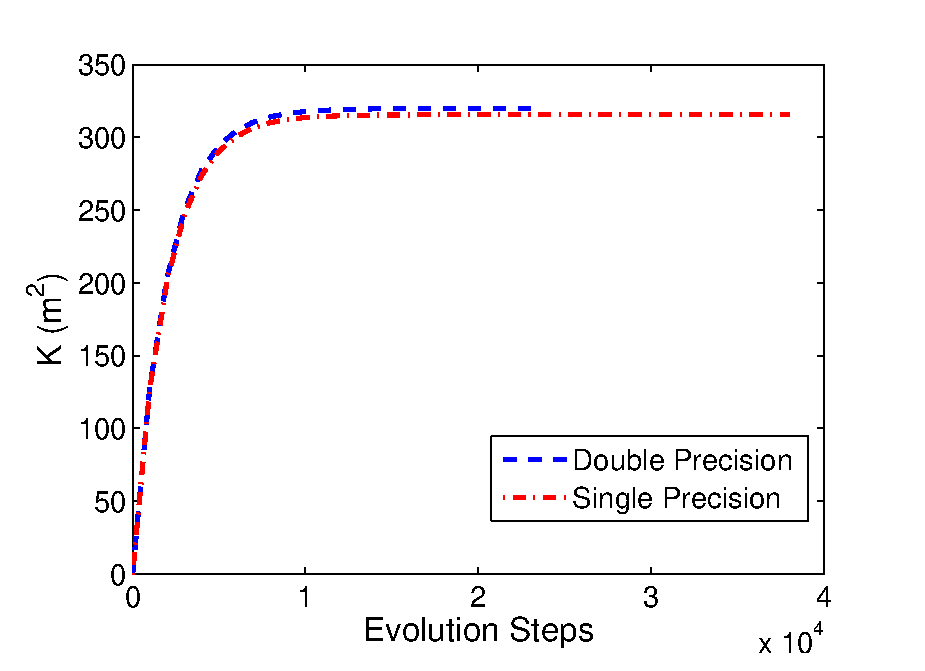
\includegraphics[width=0.6\textwidth]{img/dp_sp}
  \caption{使用单精度和双精度计算时渗透率$k$的收敛过程}
  \label{fig:dp_sp}
\end{figure}

%我们比较了二者在演化30000步之后,垂直
%于外力方向的中心截面上$\bm X$方向的速度分量(该截面位置如图\ref{fig:bcc_U}所示)。
%二者相对差别按下式计算
%\begin{equation}
  %\delta u_r =  \frac{\sqrt {\sum\nolimits_{ij}{| \bm u_{ij}^{dp}- \bm u_{ij}^{sp} |^2}}}{\sqrt{\sum\nolimits_{ij}{|  \bm u_{ij}^{dp} |^2}}}
  %\label{diff_dp_sp}
%\end{equation}
%式中上标$sp$和$dp$分别表示单精度和双精度。

\subsection{计算速度分析}
在这一小节中,我们分析各种影响计算速度的因素,包括所使用的优化算法(见5.2、5.3节)、
模型(MRT和LBGK)、计算精度、Block尺寸。在下面的比较中,如无特别指明,均采用单精度计算,Block尺寸
为64。另外,我们在4.2节中指出衡量多孔介质模拟计算速度时有两种单位\--- MLUPS
和MFLUPS,后者只统计流体格点更新,即考虑了孔隙率对计算量的影响,二者换算关系为
\begin{equation}
  Speed\text{(MFLUPS)} = \epsilon \times Speed \text{(MLUPS)}
  \label{speed_relation}
\end{equation}
在本小节的图中,我们会明确标出所使用的衡量单位。为叙述方便我们在后文中称5.2节中
中算法为算法一,而称采用5.3节中介绍的稀疏存储模式的算法为算法二。

为方便对比,我们还编写了同样计算这个问题的CPU版本程序,采用intel icc编译器编译,并加上了
\texttt{-fast}编译选项(这是目前我们所能利用的最快的编译方法),
在各种工况下观测到的最高流体格点更新速率为3.61MFLUPS。

\subsubsection{算法的影响}
图\ref{fig:speed_algo_ML}所示为采用两种算法在不同孔隙率下的计算速度,单位为MLUPS,
图\ref{fig:speed_algo_MFL}反映相同内容,不过单位为MFLUPS。
\begin{figure}[htb]
  \centering
  \subfigure[衡量单位:MLUPS:]{
    \begin{minipage}[b]{0.42\textwidth}
      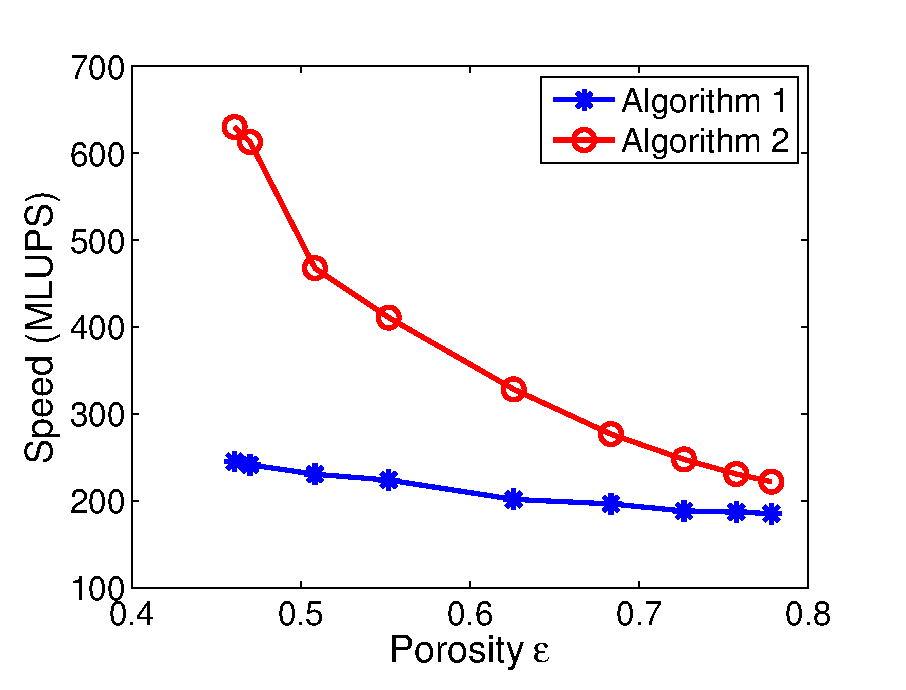
\includegraphics[width=1\textwidth]{img/speed_algo_ML}
      \label{fig:speed_algo_ML}
    \end{minipage}
  }
  %\hspace{2em}
  \subfigure[衡量单位:MFLUPS]{
    \begin{minipage}[b]{0.42\textwidth}
      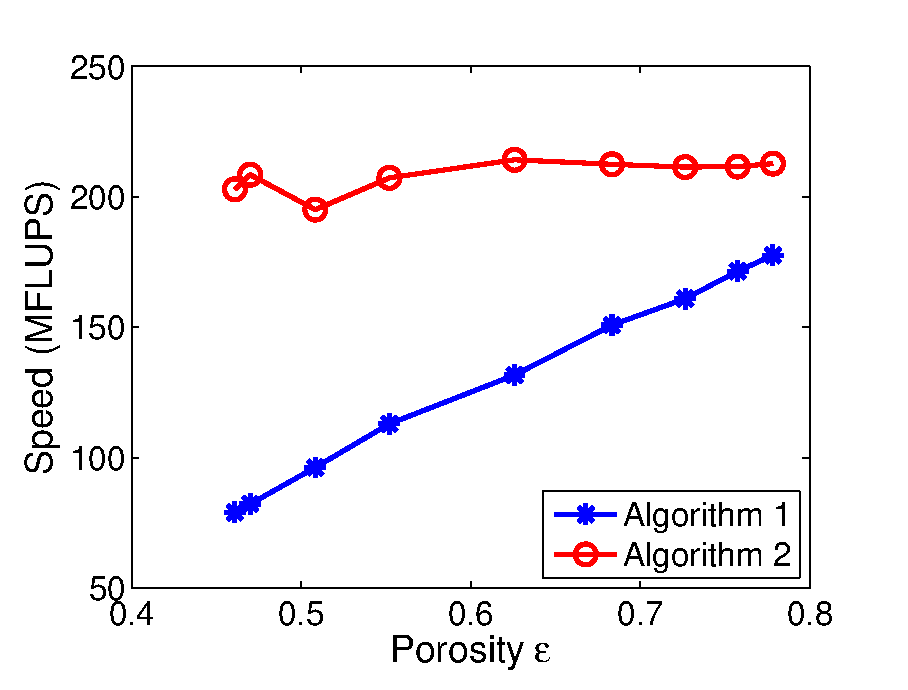
\includegraphics[width=1\textwidth]{img/speed_algo_MFL}
      \label{fig:speed_algo_MFL}
    \end{minipage}
  }
  \caption{算法对计算速度的影响}
\end{figure}
对比图\ref{fig:speed_algo_ML}中的红线和蓝线可以发现,随着孔隙率减小,采用算法二
格点更新速度大幅提高,而采用算法一则速度只有很小的提高,并且在所考差的孔隙率范围
内算法二格点计算速度均优于算法一。对比\ref{fig:speed_algo_ML}中的红线和蓝线可以发现,
随着孔隙率减小,算法一的流体格点更新速度几乎线性减小而算法二则没有显著变化,我们分析
这是因为采用算法一时,同一个wrap中的每个无效格点(固体)虽然不参与计算,但也
占据了SP执行时间。

\subsubsection{MRT和LBGK模型的影响}
MRT模型相对于BGK模型只在计算量上有所增加,而访存模式即访存大小都没有变化。通常
文献中反映其计算量约增加了$15\%\sim20\%$\ucite{guoredbook}。这里我们分析了
采用算法一时两者的计算速度的差别,其结果见图\ref{fig:speed_model},图中所示
为在不同孔隙率下采用MRT模型计算速度相对LBGK模型的下降量,可以发现相对下降量
都小于10\%。
\begin{figure}[htb]
  \centering
  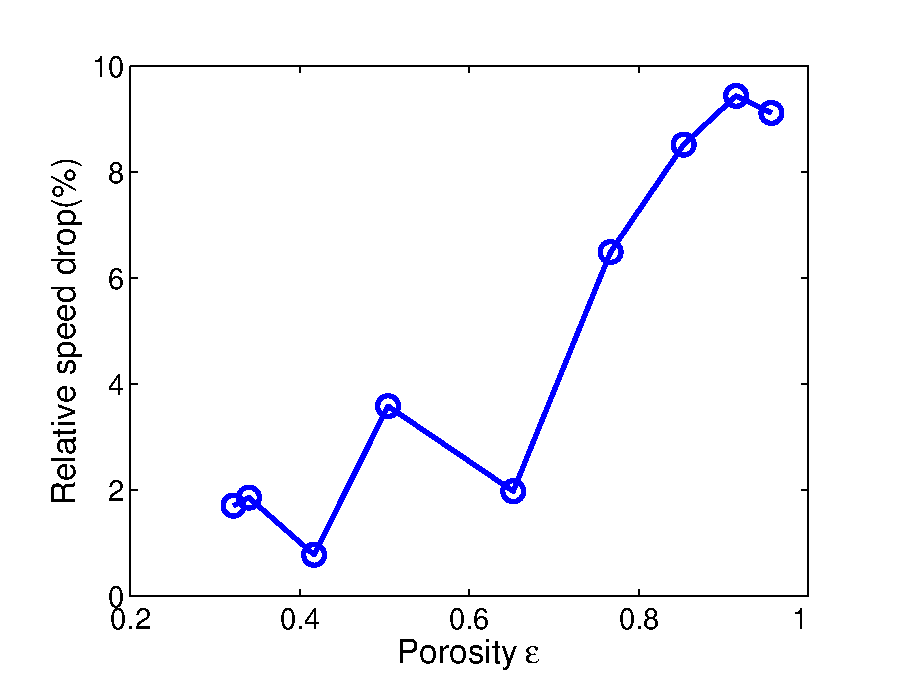
\includegraphics[width=0.6\textwidth]{img/speed_model}
  \caption{MRT模型相对LBGK模型计算速度的相对下降量}
  \label{fig:speed_model}
\end{figure}

\subsubsection{单、双精度的影响}
我们采用算法一结合MRT模型比较了单、双精度的计算速度,结果如图\ref{fig:speed_dpsp}所示,
可以发现双精度计算速度为单精度的34\%左右。在我们所使用的Tesla C1060 GPU上,双精度计算
速度理论上是单精度的$1/12$,而此处34\%与之相差较大,我们分析这是因为LB的计算性能瓶颈在
显存带宽而不在处理器执行速度,双精度计算相对单精度带宽需求只增大一倍,考虑到其他因素
如访存效率影响,此处43\%在预期范围内。
\begin{figure}[htb]
  \centering
  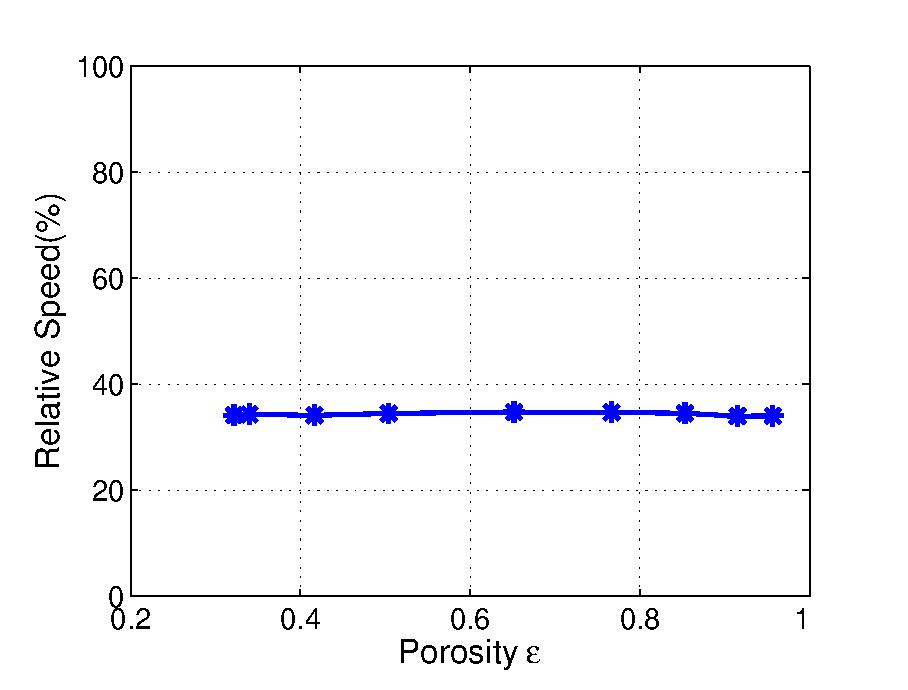
\includegraphics[width=0.6\textwidth]{img/speed_dpsp}
  \caption{双精度相对单精度的计算速度}
  \label{fig:speed_dpsp}
\end{figure}

\subsubsection{Block尺寸的影响}
上面的速度测试Block大小都是64, 这里我们分别测试了Block大小为96和128时的计算速度。
采用的的模型和算法分别是MRT模型与算法二。
结果见图\ref{fig:speed_block},可以发现Block大小为64时速度最高,而为96和128时
速度较小且差别不大,这是定型的计算效率受到寄存器或共享内存数量限制的现象。
考虑到我们Kernel只使用了寄存器,而没有使用共享内存,所以此处Block尺寸增大时,性能
下降的现象应该是性能受到寄存器数量的限制引起的。
\begin{figure}[htb]
  \centering
  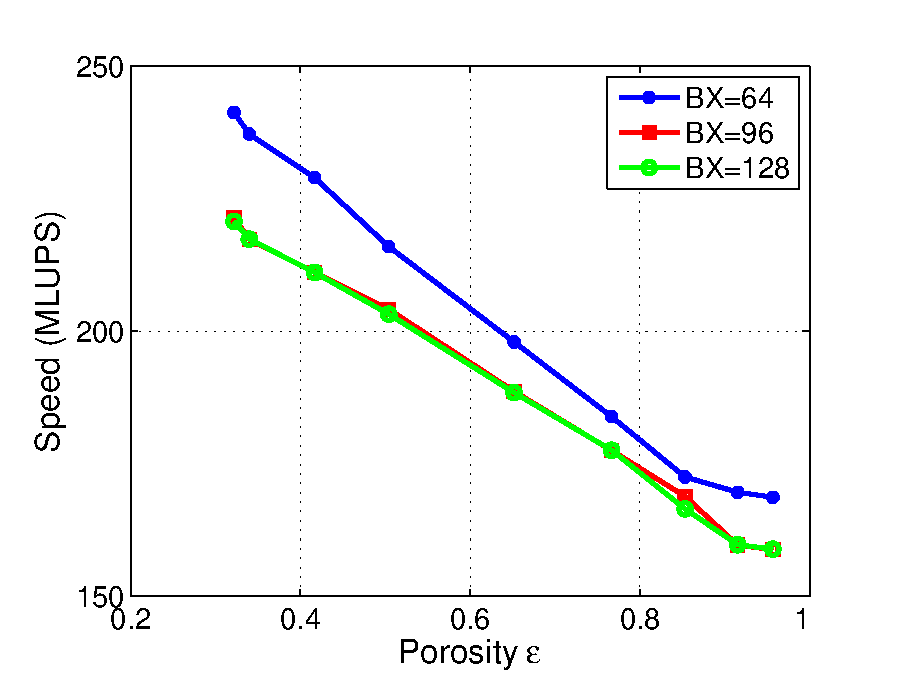
\includegraphics[width=0.6\textwidth]{img/speed_block}
  \caption{不同Block大小时的计算速度}
  \label{fig:speed_block}
\end{figure}

\section{小结}
本章中我们首先介绍了LBM处理多孔介质的一般方法,
并指出了两种针对在GPU上实现多孔介质流动模拟的优化技术
\---利用位操作结合逻辑运算减小访存量和优化指令流以及利用稀疏存储模式减小
显存用量和提高程序计算速度。
随后我们分别运用这两个优化技术编制了LBGK模型和MRT模型的GPU程序计算了BCC
多孔介质模型的渗透率,与解析解对比发现吻合良好,证明了我们GPU程序实现
正确。最后我们详细分析了上述GPU程序的计算速度,详细考察了各种影响计算
速度的因素,在最优情况,我们的GPU程序计算速度可达212MFLUPS和630MLUPS。
超过CPU串行程序50倍。在下一章中我们将本章介绍的优化算法运用于更复杂的多孔介质内的多相流LBM
模拟。
